\setchapterimage[6cm]{chapter/operating_system/logo.png}
\setchapterpreamble[u]{\margintoc}
\chapter[Operating systems]{Programming languages for operating systems\protect\footnotemark}
\labch{operating-sysmets}

\footnotetext{Ubuntu 19.04 "Disco Dingo" Author: \href{https://commons.wikimedia.org/wiki/File:Ubuntu_19.04_\%22Disco_Dingo\%22.png}{JulianVilla26 / 2019 / GNU General Public License}.}

The chapter explores the object of the <<operating system>> and its properties. The following problems were solved in the paper with the help of SPARQL queries: finding instances of the object <<operating system>>, building a list of operating systems (OS) by base, by creation time, by programming language, in which the OS was written. Also a histogram is constructed, it shows the number of programs written in some programming language, and the proportion of how many of them work for some OS. A lot of software does not specify the programming language on which it was developed. The property <<programming language>> was added to several objects to improve the results.

\section{Instances of the object "operating system"}

Let's build a list of all the operating systems.

\begin{lstlisting}[ language=SPARQL, 
caption={List of operating systems\\\hspace{\textwidth} 
SPARQL query \num{510} results (January 2018), \num{1086} results (September 2020).
SPARQL query: \href{https://w.wiki/nDb}{https://w.wiki/nDb}
},
label=lst:all_operating_systems,
texcl 
]
SELECT ?os ?osLabel
WHERE
{
	?os wdt:P31 wd:Q9135. # instance of operating system
	SERVICE wikibase:label { bd:serviceParam wikibase:language "en" }
}
\end{lstlisting}

The most complete and detailed operating systems on Wikidata are: \wdqName{Linux}{388}, \wdqName{Microsoft Windows}{1406}, \wdqName{Windows 8}{5046}.

Almost empty and less informative operating systems are: \wdqName{SPIN}{16314510}, \wdqName{JavaOS}{1684163}, \wdqName{Atari TOS}{1574899}, \wdqName{Xubuntu}{72688}.

According to ProWD the only one Russian operating system on Wikidata is Miraculix, which has 7 properties. The leaders in terms of the number of properties (24 properties) among operating systems around the world are \wdqName{Microsoft Windows}{1406} and \wdqName{Windows 8}{5046}.

\section{Operating systems bases}
Listing \ref{lst:base_of_operating_systems} shows a SPARQL query to list the \href{https://www.wikidata.org/wiki/Property_talk:P144}{P144 base} operating systems. This query shows the correspondence between the "Operating System" and its "ancestor" on which it is based.

\marginnote{
	Select the operating system that has the most other operating systems:
	\begin{itemize}
		\item \href{https://w.wiki/n8U}{Debian}
		\item \href{https://w.wiki/n8V}{Android}
		\item \href{https://w.wiki/n8W}{Ubuntu}
		\item \href{https://w.wiki/n8X}{Linux kernel}
	\end{itemize}
%	Answer at~\ref{answer:what_system_created} on page~\pageref{answer:what_system_created}.
}

\begin{lstlisting}[ language=SPARQL, 
caption={List of operating systems by base\\\hspace{\textwidth}
SPARQL query \num{159} results (January 2018), \num{118} results (September 2020).
SPARQL query: \href{https://w.wiki/nDc}{https://w.wiki/nDc}
},
label=lst:base_of_operating_systems,
texcl 
]
SELECT ?osLabel ?baseLabel
WHERE
{
	?os wdt:P31 wd:Q9135. # inctance of operating system
	?os wdt:P144 ?base. # os is based on 
	SERVICE wikibase:label { bd:serviceParam wikibase:language "en" }
}
GROUP BY ?osLabel ?baseLabel
\end{lstlisting}

\section{Operating systems release dates}
\marginnote{
	Which of these operating systems:
	\href{https://w.wiki/n8P}{Newton OS},
	\href{https://w.wiki/n8Q}{Ubuntu Touch},
	\href{https://w.wiki/n8R}{JavaOS};
	\href{https://w.wiki/n8S}{Apple} developed?
%	Answer at~\ref{answer:what_system_created} on page~\pageref{answer:what_system_created}.
}

Listing \ref{lst:inception_time_of_operating_systems} shows a SPARQL query to get a list of operating systems with their creation date.

\begin{lstlisting}[ language=SPARQL, 
caption={List of operating systems by creation time\\\hspace{\textwidth}
SPARQL query \num{298} results (2018), \num{238} results (2020).
SPARQL query: \href{https://w.wiki/nDf}{https://w.wiki/nDf}
},
label=lst:inception_time_of_operating_systems,
texcl 
]
#defaultView:Timeline
SELECT ?osLabel ?time
WHERE
{
	?os wdt:P31 wd:Q9135. # inctance of operating system
	?os wdt:P571 ?time. # created at
	SERVICE wikibase:label { bd:serviceParam wikibase:language "en" }
}
GROUP BY ?osLabel ?time
ORDER BY DESC(?time)
\end{lstlisting}

Listing \ref{lst:inception_time_of_operating_systems} shows in a nice graphical shell (figure \ref{fig:os_creation}) a timeline for creating (actually release) operating systems. And it also shows how poorly Wikidata is filled, since only 230 results are displayed in queries in 2020. Which, in turn, means that for other "objects" the field "date of creation" is simply not filled. Although the information about the "release date" is not so secret.

\begin{figure*}[h!]
	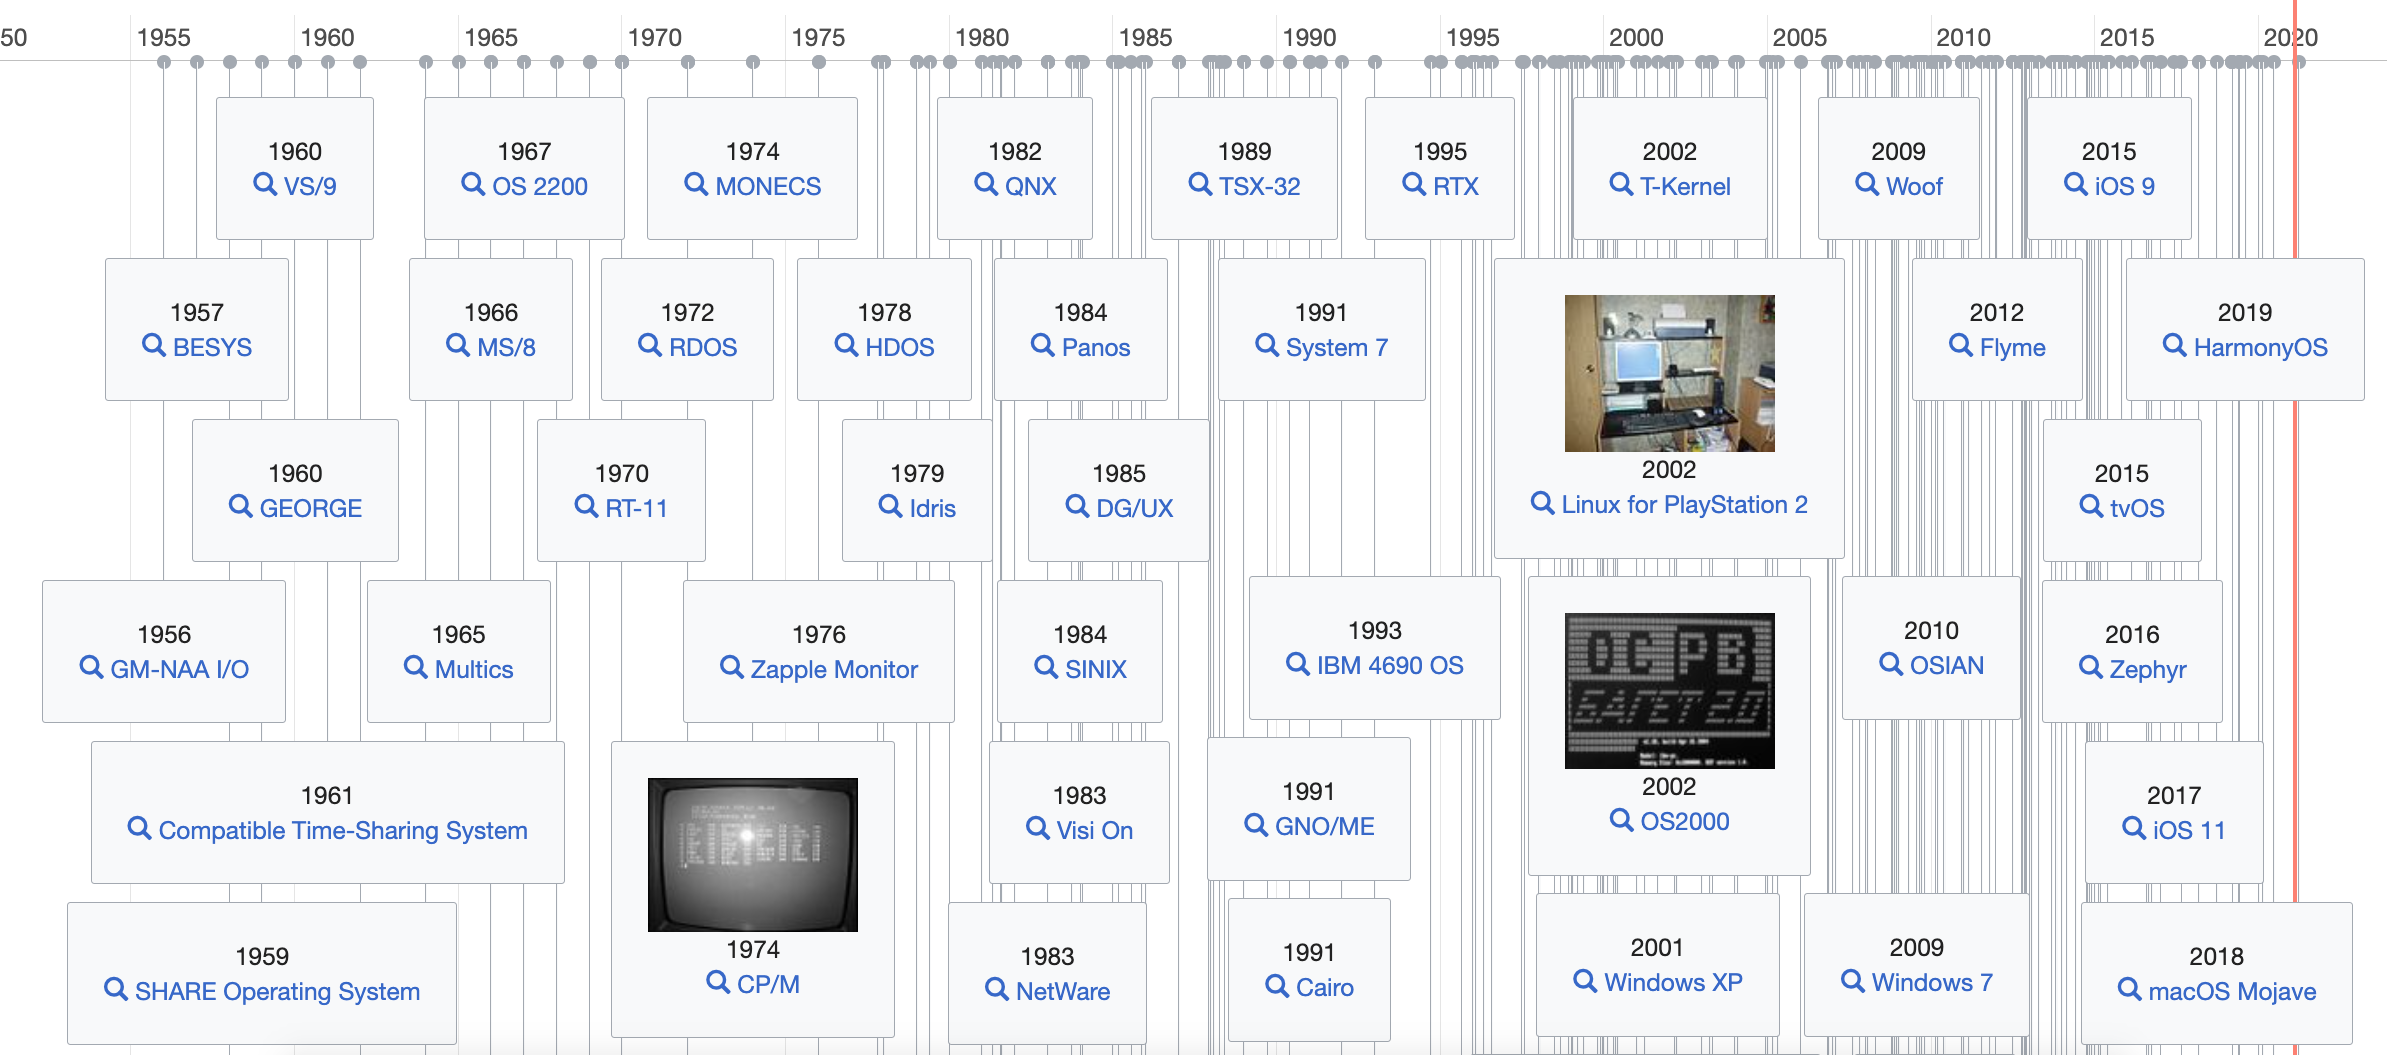
\includegraphics{./chapter/operating_system/os-creation.png}
	\caption{Part of the operating system release timeline for 2020 year.}
	\label{fig:os_creation}
\end{figure*}

\section{Operating systems with programming language}

Listing \ref{lst:count_os_on_languages} shows a SPARQL query to get a list of programming languages with the output of the number of operating systems written in them.

\begin{lstlisting}[ language=SPARQL, 
caption={Count of operating systems by programming language\\\hspace{\textwidth}
SPARQL query \num{35} results (January 2018), \num{37} results (September 2020).
SPARQL query: \href{https://w.wiki/nDh}{https://w.wiki/nDh}
},
label=lst:count_os_on_languages,
texcl 
]
SELECT ?lang (count(*) as ?count)
WHERE 
{
	?os wdt:P31 wd:Q9135. # instance of operating system
	?os wdt:P277 ?langObj. # created on programming language
	OPTIONAL {
		?langObj rdfs:label ?lang
		filter (lang(?lang) = "ru")
	}
}
GROUP BY ?lang
ORDER BY DESC(?count) ASC(?lang)
\end{lstlisting}

The query shows (only on the basis of the completed wikis, so it's not a fact that it's true) that the OS is predominantly written in Assembler language, which is certainly true, because it is the fastest, yet convenient programming language. On the second and third places are C and C++, which are not the worst analogue, because in spite of its "slowness", they are the most convenient and simple programming languages.

\section{Programming languages used to write operating systems}
If you look at the number of operating systems for which the property "programming language" is specified, you can see that from \num{1086} objects this property is filled only in \num{116}. But according to the data for 2020, presented in fig.~\ref{fig:count-os-written-on-languages}, it can be determined that most operating systems are written in the C programming language, namely 44 operating systems.

\begin{figure*}[h!]
	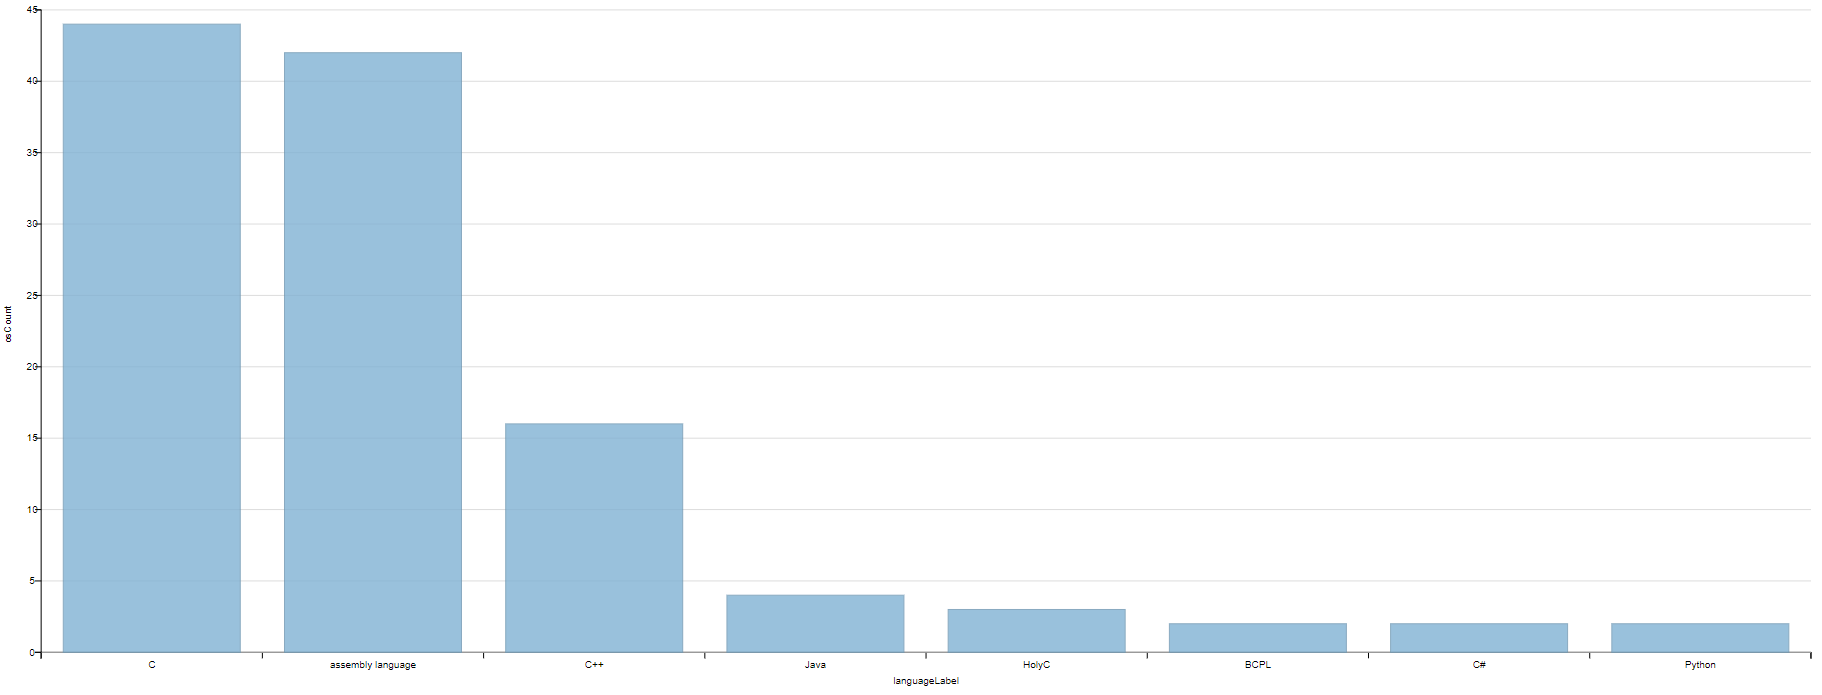
\includegraphics{./chapter/operating_system/count-os-written-on-languages.png}
	\caption{Count of operating systems which written by programming language (2020).}
	\label{fig:count-os-written-on-languages}
\end{figure*}


\section{The amount of software for each OS in how many languages is it written}
Listing \ref{lst:count_soft_on_os} shows a SPARQL query showing for each software for each OS, in how many languages it is written.

\begin{lstlisting}[ language=SPARQL, 
	caption={List of OS with the amount of software for it\\\hspace{\textwidth}
		SPARQL query \num{2259} results (2018), \num{6883} results (2020).
		SPARQL query: \href{https://w.wiki/n8C}{https://w.wiki/n8C}
	},
	label=lst:count_soft_on_os,
	texcl 
	]
	SELECT ?soft ?softLabel ?os ?osLabel (count(*) as ?count)
	WHERE
	{
		?soft wdt:P306 ?os. # operating system on which a software works
		?soft wdt:P277 ?lang. # programming language in which soft is developed
		SERVICE wikibase:label { bd:serviceParam wikibase:language "ru, en" }
	}
	GROUP BY ?soft ?softLabel ?os ?osLabel
	ORDER BY DESC(?count) ASC(?lang)
\end{lstlisting}


\section{How much software was written for the OS using a particular language}
Listing \ref{lst:count_soft_on_os_with_lang} presents a SPARQL query showing for each software for each OS in how many languages it is written.

\begin{lstlisting}[ language=SPARQL, 
	caption={List of programming languages with the amount of software written for it\\\hspace{\textwidth}
		SPARQL query \num{2259} results (2018), \num{6883} results (2020).
		SPARQL query: \href{https://w.wiki/n8D}{https://w.wiki/n8D}
	},
	label=lst:count_soft_on_os_with_lang,
	texcl 
	]
	SELECT ?osLabel ?softLanguageLabel (count(*) as ?count)
	WHERE
	{
		?soft wdt:P306 ?os. # software works on os
		?soft wdt:P277 ?softLanguage. # software is written 
									# by programming language
		?os wdt:P277 ?osLanguage. # os is written by programming language
		SERVICE wikibase:label { bd:serviceParam wikibase:language "ru, en"}
	}
	GROUP BY ?osLabel ?softLanguageLabel
	ORDER BY DESC(?count) DESC(?osLabel)
\end{lstlisting}

This request perfectly shows that most of the software written for \href{https://www.wikidata.org/wiki/Q14116}{macOS} is written in \href{https://www.wikidata.org/wiki/Q2407}{C++} (374 programs), \href{https://www.wikidata.org/wiki/Q15777}{C} (276 programs), \href{https://www.wikidata.org/wiki/Q28865}{Python} (107 programs).
For \href{https://www.wikidata.org/wiki/Q94}{Android} -- \href{https://www.wikidata.org/wiki/Q2407}{C++} (107 programs) and \href{https://www.wikidata.org/wiki/Q251}{Java} (80 programs).
For \href{https://www.wikidata.org/wiki/Q48493}{iOS} -- \href{https://www.wikidata.org/wiki/Q2407}{C++} (63 programs).


The histogram in the fig.~\ref{fig:count-software-written-on-languages} allows you to see for each programming language the number of programs that have been written in it, as well as under what OS these programs work. The graph shows that the largest number of programs is written in languages. \href{https://www.wikidata.org/wiki/Q2407}{C++} (2503 programs), 
\href{https://www.wikidata.org/wiki/Q15777}{C} (2566 programs), 
\href{https://www.wikidata.org/wiki/Q251}{Java} (799 programs),
\href{https://www.wikidata.org/wiki/Q28865}{Python} (717 programs),
\href{https://www.wikidata.org/wiki/Q2005}{Javascrip} (344 programs).


\begin{figure*}[h!]
	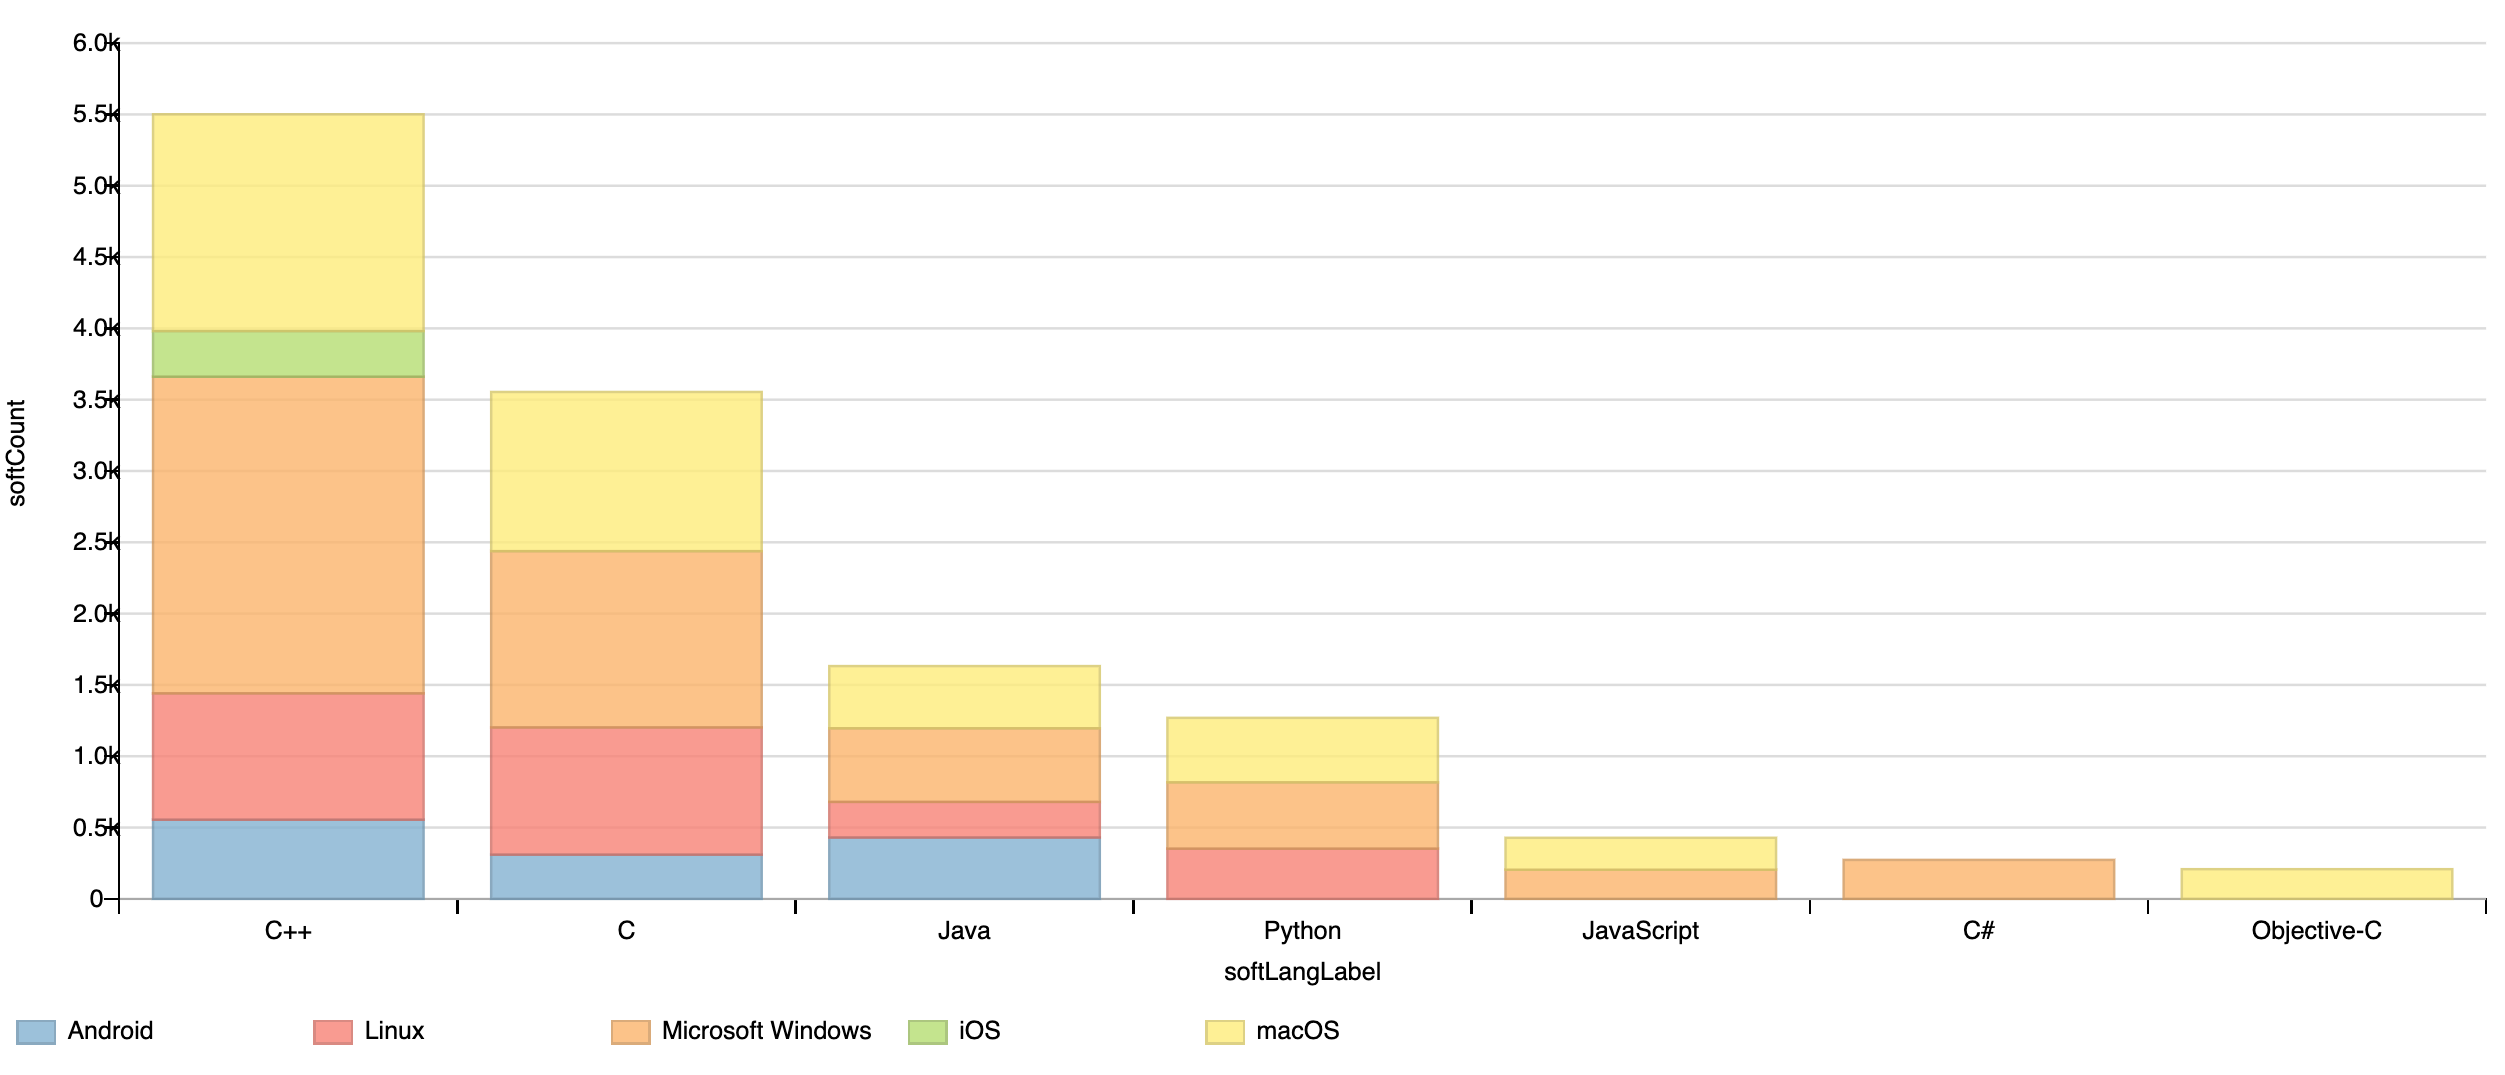
\includegraphics{./chapter/operating_system/Programming-languages-and-count-of-programms-written-on-them-and-OS-2020.png}
	\caption{Programming languages and count of OSs for which programs written in languages (2020).}
	\label{fig:count-software-written-on-languages}
\end{figure*}

Let's consider each of these languages in more detail.

Most of the C ++ programs are written for Windows (472 programs) and macOs (300 programs). Despite the fact that the C ++ language was developed in 1972, it has not yet lost its popularity due, probably, to the fact that it is used to write low-level applications, since it is inferior in "proximity" to the hardware level, perhaps, to the assembler.

Most of the programs in C ++ are written for macOS (400 programs) and Windows (700 programs) and Linux (400 programs). Probably, C ++ will lead for a long time, since at the moment it is used for solutions that require high performance, which is not allowed by high-level languages like Java or C\#.

Most Java programs are written for macOS (196 programs) and Android (156 programs). Java is probably popular because of its portability\footnotemark \footnotetext{Portability - the ability to run code on multiple platforms without any changes.}
code, that is, Java code will run on any machine with the JVM\footnotemark installed.
\footnotetext{The Java virtual machine (JVM) is a program designed to run other programs.}

Most JavaScript programs are written for macOS (100 programs) and Android (60 programs) and iOS (40 programs). As a rule, it is used to write the client-side of web applications that the development of complex web applications leads to a decrease in the load on the server and an increase in the speed of the application.

Most Python programs are written for macOS (212 programs) and Linux (107 programs). Used, for example, for writing web applications and data analysis.

Looking at the histogram, we can conclude that each of the languages considered has occupied its own "niche" in the field of software development and is used for a certain range of tasks. It is also important to note that most of the software is written for macOS (900 programs), Windows (1500 programs), Linux (1200 programs) or Android (300 programs).